\documentclass{amsart}

\usepackage{subfiles}

% Packages
\usepackage{mathtools}
\usepackage{amssymb,bm,bbold}
\usepackage{enumerate}
\usepackage{lipsum}
\usepackage[dvipsnames]{xcolor}
\usepackage{tikz}
\usepackage{caption}
\usepackage{subcaption}

% hyperref
\usepackage{hyperref}
\usepackage{cleveref}
\newcommand\myshade{90}
\colorlet{mylinkcolor}{MidnightBlue}
\colorlet{mycitecolor}{Cerulean}
\colorlet{myurlcolor}{Cerulean}

\hypersetup{
  linkcolor  = mylinkcolor!\myshade!black,
  citecolor  = mycitecolor!\myshade!black,
  urlcolor   = myurlcolor!\myshade!black,
  colorlinks = true,
}

% Bibliography
\usepackage[
backend=biber,
style=alphabetic,
sorting=ynt
]{biblatex}

\addbibresource{bibliography.bib}

% counters
\newcounter{example}[section]
\newenvironment{example}[1][]{\refstepcounter{example}\par\medskip
   \noindent \textbf{Example~\theexample. #1} \rmfamily}{\medskip}
\newcounter{definition}[section]
\newenvironment{definition}[1][]{\refstepcounter{definition}\par\medskip
   \noindent \textbf{Definition~\thedefinition. #1} \rmfamily}{\medskip}
\newcounter{question}[section]
\newenvironment{question}[1][]{\refstepcounter{question}\par\medskip
   \noindent \textbf{Question~\thequestion. #1} \rmfamily}{\medskip}

% theorem environments
\usepackage{amsthm}
\newtheorem{theorem}{Theorem}[section]
\newtheorem{corollary}{Corollary}[theorem]
\newtheorem{lemma}{Lemma}[section]
\newtheorem{problem}{Problem}
\newenvironment{solution}{\paragraph{\textit{Solution}}}{\hfill$\square$}

\usepackage{listings}

% convenient notations
\newcommand{\NN}{\mathbb{N}} % Naturals
\newcommand{\CC}{\mathbb{C}} % Complex numbers
\newcommand{\QQ}{\mathbb{Q}} % Rationals
\newcommand{\RR}{\mathbb{R}} % Reals
\newcommand{\ZZ}{\mathbb{Z}} % Integers
\newcommand{\EE}{\mathbb{E}} % Expectation
\newcommand{\PP}{\mathbb{P}} % Probability
\newcommand{\Epsilon}{\mathcal{E}}
\newcommand{\nsum}{\sum_{i=1}^n}

\newcommand{\floor}[1]{\left\lfloor{#1}\right\rfloor}
\newcommand{\ceil}[1]{\left\lceil{#1}\right\rceil}
\newcommand{\norm}[1]{\left\lVert{#1}\right\rVert}
\newcommand{\diff}{\operatorname{diff }}
\newcommand{\disc}{\operatorname{disc }}
\newcommand{\ord}{\operatorname{ord}}
\newcommand{\lcm}{\operatorname{lcm}}
\newcommand{\del}{\partial}
\newcommand{\emp}{\varnothing}
\newcommand{\divides}{\,|\,}
\newcommand{\op}[1]{\operatorname{#1}}
\newcommand{\mf}[1]{\mathfrak{#1}}
\newcommand{\mc}[1]{\mathcal{#1}}

\DeclareMathOperator*{\argmax}{arg\,max}
\DeclareMathOperator*{\argmin}{arg\,min}

% % % % % % % % % % % % % % % % % % % % % % % % % % % % % % % % % % % % % % % % % % % % % % % % % % % % % % % %
% Typography, change document font
\usepackage[tt=false, type1=true]{libertine}
\usepackage[varqu]{zi4}
\usepackage[T1]{fontenc}

%%
%% Julia definition (c) 2014 Jubobs
%%

\definecolor{backcolour}{rgb}{0.95,0.95,0.92}
\lstdefinelanguage{Julia}
  {morekeywords={abstract,break,case,catch,const,continue,do,else,elseif,%
      end,export,false,for,function,immutable,import,importall,if,in,%
      macro,module,otherwise,quote,return,switch,true,try,type,typealias,%
      using,while},
   sensitive=true,
   alsoother={$},
   morecomment=[l]\#,
   morecomment=[n]{\#=}{=\#},
   morestring=[s]{"}{"},
   morestring=[m]{'}{'},
}[keywords,comments,strings]

\lstset{
    language          = Julia,
    backgroundcolor   = \color{white},
    basicstyle        = \ttfamily\tiny,
    keywordstyle      = \bfseries\color{MidnightBlue},
    stringstyle       = \color{Cerulean},
    commentstyle      = \color{Gray},
    numberstyle       = \tiny\color{Gray},
    breakatwhitespace = false,
    captionpos        = t,
    numbers           = left,
    numbersep         = 5pt,
    showspaces        = false,
    showstringspaces  = false,
    showtabs          = false,
    tabsize           = 2,
}

\usepackage{algorithm}
\usepackage{algpseudocode}

% Disable paragraph indentation, and increase gap
\usepackage{parskip}

\title{APMA2560 Final Project: Topology Optimization}
\author{Matthew Meeker}
\begin{document}
\maketitle

\section{Introduction}

Briefly, topology optimization offers a class of techniques and algorithms for discovering the optimal distribution of
material within a given domain, subject to some set of physics and other constraints, which tend to form
PDE-constrained optimization problems. In general, these problems take the form
\begin{equation}\label{eq:general_problem}
    \begin{aligned}
        \min_{\rho} &\quad F = F(u(\rho), \rho)=\int_\Omega f(u(\rho), \rho)\mathrm{d}V\\
        \text{s.t.} &\quad \int_\Omega \rho \mathrm{d}V - V_0 \leq 0,\\
         &\quad G_i(u(\rho), \rho) \leq 0,
    \end{aligned}
\end{equation}
where $\Omega$ is the design domain, $\rho \in L^2(\Omega)$ is a function describing the material distribution,
$f$ forms the objective function, $\theta$ is the \textit{mass fraction} (that is, the fraction of $\Omega$
which may be occupied by material; this may be made physical by considering material cost constraints, etc.),
and $G_j$ describes a related set of constraints.

\tableofcontents

\section{Classical Methods}
Like the finite element method itself, Topology Optimization found its first motivations in mechanical engineering;
for this reason, the classic problem is to construct a stiff structure in the design domain that minimizes the
\textit{compliance} (or, strain energy) under the given boundary conditions.

In the ideal, we would be able to 


\section{Structural Compliance with \texttt{top88}}
As a first example problem, we will consider structural compliance and the method given in \cite{andreassen_clausen_schevenels_lazarov_sigmund_2010}.
A Julia implementation of the code may be found in the appendices.

The MBB beam is a classic problem from mechanical engineering for topology optimization. Within $\Omega$,
subject to natural constraints on cost and area, we would like to build a maximally stiff structure.
Intuition would serve a solution with stacked triangles, as will be observed.

\begin{figure}
    \centering
    \caption{$\Omega$ for \texttt{top88.jl} with the applied boundary conditions and loads.}
    \includegraphics[width=\textwidth]{imgs/Top88/problem_diagram.png}
\end{figure}

\subsection{Problem Specification}

The domain $\Omega$ is discretized with (square) quadrilateral elements and the density approach is adopted,
so, to each element $e$ in the domain, we will associate a material density $x_e$ that is used to determine
its Young's modulus $E_e$ by
\begin{equation}
    E_e(x_e) = E_{\text{min}} + x_e^p (E_0 - E_{\text{min}}).
\end{equation}
As mentioned, $p$ is typically taken to be $3$ and $E_{\text{min}}$ is a relatively very small value
that is assigned to all elements for primarily numerical reasons -- in particular, we avoid running into
a singualr stiffness matrix. \cite{andreassen_clausen_schevenels_lazarov_sigmund_2010} titles this a
``modified SIMP approach.'' Following the format of \autoref{eq:general_continuous}, the problem may be
written
\begin{equation}\label{eq:top88_problem}
    \begin{aligned}
        \min_{\mathbf{x}} &\quad c(\mathbf{x}) := U^T K U = \sum E_e(x_e) u_e^T k_0 u_e\\
        \text{s.t.} &\quad V(x)/ V_0 = \theta,\\
            &\quad KU = F,\\
            &\quad 0 \leq \rho \leq 1.
    \end{aligned}
\end{equation}
Here, $c$ defines the compliance, $U$ and $F$ denote resp. the global displacement and force vectors, $K$
is the global stiffness matrix, $u_e$ is the element displacement vector, $k_0$ is the element stiffness
matrix (for a unit Young's modulus), and $\mathbf{x}$ denotes the element densities/ material distribution.
Lastly, $V(x)$ denotes the volume of $x$, $V_0$ of the entire domain $\Omega$, and $\theta$ is a prescribed
volume fraction (ie, the fraction of the design domain the structure is allowed to take up).

\subsubsection{Optimality Criteria Method}

The optimization problem is solved with a standard optimality criteria method.
\begin{equation}
    x_e^{t+1} = \begin{cases}
        \max(0, x_e - m) & \text{if } x_e B_e^\eta \leq \max(0, x_e - m)\\
        \min(1, x_e + m) & \text{if } x_e B_e^\eta \geq \min(1, x_e + m)\\
        x_e B_e^\eta & \text{otherwise.}
    \end{cases}
\end{equation}
$m$ is a positive move limit, $\eta (= 1/2)$ is a numerical damping coefficient, and $B_e$ is obtained
from the optimality condition as
\begin{equation}
    B_e = \frac{-\frac{\partial c}{\partial x_e}}{\lambda \frac{\partial V}{\partial x_e}},
\end{equation}
where the Lagrangian multiplier $\lambda$ must be chosen such that the volume constraint is satisfied, which
can be found with a bisection algorithm.

The partials of the objective function $c$ and material volume $V$ with respect to $x_e$ are
\begin{equation}
    \frac{\partial c}{\partial x_e} = -p x_e^{p-1} (E_0 - E_{\text{min}}) u_e^T k_0 u,
\end{equation}
and
\begin{equation}
    \frac{\partial V}{\partial x_e} = 1,
\end{equation}
which comes from the assumption that each element has unit volume (so, observe that a decrease in density at
one element will lead to an equal increase in density at another element such that the volume of the structure
overall has not shifted).

\subsubsection{Filtering}

The code implements both a density and a sensitivity filter, and the filtered densities are output.

\subsection{Result}

Confirming roughly our intuition, we see a number of triangles forming. The following was run on a rectangle
of 150x50 elements with a volume fraction of $0.5$, $r_{\text{min}} / V(e) = 2.0$ (ie, radius divided by element volume),
and using a density filter.

\begin{figure}[H]
    \centering
    \caption{\texttt{top88} solution on 150x50 rectangle.}
    \includegraphics[width=\textwidth]{imgs/Top88/r150x50_density.png}
\end{figure}
\section{Thermal Compliance with \texttt{toph}}
Using an identical algorithm, we will now solve a thermal compliance problem
that will be revisited with EFEM in \autoref{sec:thermal_compliance_classic_unit_square};
the algorithm, implementation, and derivation are worked out in greater detail in \autoref{sec:toph_appendix}.

\begin{figure}[ht]
    \centering
    \caption[b]{$\Omega$ for \texttt{toph}.}
    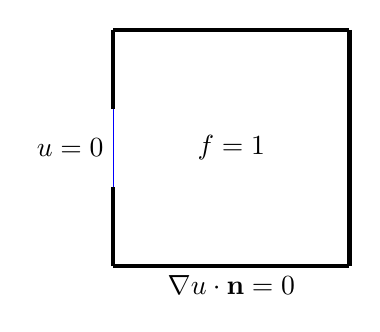
\begin{tikzpicture}
        \draw [ultra thick] (0,0) -- (0,1);
        \draw [blue] (0,1) -- (0,2);
        \draw [ultra thick] (0,2) -- (0,3);
        \draw [ultra thick] (3,3) -- (0,3);
        \draw [ultra thick] (0,0) -- (3,0);
        \draw [ultra thick] (3,3) -- (3,0);

        \node at (0, 1.5) [anchor = east] {$u = 0$};
        \node at (1.5, 1.5) {$f = 1$};
        \node at (1.5, 0) [anchor = north] {$\nabla u \cdot \mathbf{n} = 0$};
    \end{tikzpicture}
\end{figure}

That is, $\Omega$ is a square with a small component of the left side cut out allowing heat to flow through;
the interior of the domain is evenly heated. We again discretize with square elements.

\subsection{Results}

First with a 40x40 square discretization, mass fraction $\theta = 0.4$, SIMP penalization exponent of $3.0$,
and $r_\text{min}$ of 1.2, and secondly with an 80x80 square.

Keeping the constant even heating in mind, the solution reached is fairly natural: the goal
is essentially to a build a heatsink that draws heat from $\Omega$ out to the left. So, the
tree structure formed first serves this purpose as a conductor and secondly maximizes the surface area
(which can be seen as the mesh is refined).
\vfill\pagebreak

\begin{figure}[H]
    \centering
    \caption{40x40 \texttt{toph} simulation.}
    \includegraphics[width=0.8\textwidth]{imgs/TopH/toph_1.png}
\end{figure}

\begin{figure}[H]
    \centering
    \caption{80x80 \texttt{toph} simulation.}
    \includegraphics[width=0.8\textwidth]{imgs/TopH/toph_2.png}
\end{figure}





%%%%%%%%%%%%%%%%%%%%%%%%%%%%%%%%%%%%%%%%%%%%%%%%%%%%%%%%%%%%%%%%%%%%%%%%%%%%%%%%%
\section{Thermal Compliance with the Entropic Finite Element Method (EFEM)}
We would like to solve the thermal compliance problem
\begin{equation}\label{eq:thermal_compliance_problem}
    \begin{aligned}
        \min_{\rho} &\quad \int_\Omega f \cdot u \ \mathrm{d}x\\
        \text{s.t.} &\\
        &\quad\begin{cases}
            -\nabla \cdot (r(\tilde{\rho}) \nabla u) = f & \text{in } \Omega \text{ and BCs},\\
            - \epsilon^2 \Delta \tilde{\rho} + \tilde{\rho} = \rho & \text{in } \Omega \text{ and Neumann BCs},\\
            0 \leq \rho \leq 1 & \text{in } \Omega,\\
            \int_\Omega \rho\ \mathrm{d} x = \theta\cdot\text{vol}(\Omega),
        \end{cases}
    \end{aligned}
\end{equation}
over $u \in [H^1(\Omega)]^2$ and $\rho \in L^2(\Omega)$. Here, $r(\tilde{\rho}) = \rho_0 + \tilde{\rho}^3(1 - \rho_0)$
is the SIMP law,\\ $\epsilon$ is the design length scale, and $0 < \theta < 1$ is the volume fraction. Recall the
second constraint as the density filter for length parameter $\epsilon$.

\subsection{Method}

Breaking from the methodology in \texttt{toph.jl}, we will now use Keith and Surowiec's Entropic Mirror Descent algorithm (2023)
tailored to the constraint $\rho \in [0,1]$. Below, we will let $\sigma$ denote the sigmoid function, $\sigma^{-1}$
the inverse sigmoid function,
$\text{clip(y)} := \min(\text{max\_val}, \max(\text{min\_val}, y))$, and $\text{projit}(\psi)$ is a (compatible) projection
operator yet to be defined.

\begin{algorithm}
    \caption{Entropic Mirror Descent for PDE-constrained Topology Optimization}\label{alg:EMD}
    \begin{algorithmic}
    \Require $\mathcal{L}(u, \rho, \tilde{\rho}, w, \tilde{w})$ (the Lagrangian), $\alpha > 0$ (the step size)
    \Ensure $\rho = \argmin \int_\Omega f \cdot u \ \mathrm{d}x$
    \State $\psi \gets \sigma^{-1}(\theta)$ \Comment{So that $\int \sigma(\psi) = \theta \cdot \text{vol}(\Omega)$}
    \While{not converged}

        $\tilde{\rho} \gets$ solution to $\partial_{\tilde{w}} \mathcal{L} = 0$, \Comment{Filter solve}

        $u \gets$ state solution; solution to $\partial_{w} \mathcal{L} = 0$, \Comment{Primal problem}

        $\tilde{w} \gets$ filtered gradient; solution to $\partial_{\tilde{\rho}} \mathcal{L} = 0$,

        $G \gets M^{-1} \tilde{w}$; ie, is the solution to $(G,v) = (\tilde{w}, v)$ for all $v \in L^2$,

        $\psi \gets \text{clip}(\text{projit}(\psi - \alpha G))$. \Comment{Mirror descent update}

    \EndWhile
    \end{algorithmic}
\end{algorithm}
for the following discretization choices $u \in V \subset [H^1]^d$, $\psi \in L^2$ (with $\rho = \sigma(\psi)$),
$\tilde{\rho} \in H^1$, $w \in V$, $\tilde{w} \in H^1$, where
\begin{algorithm}
    \caption{projit($\psi$) Nonlinear Projection}
    \begin{algorithmic}
        \Require $\psi \in L^2(\Omega)$, $0 < \theta < 1$
        \Ensure $\int_{\Omega} \sigma(\psi + c)\ \mathrm{d}x = \theta \cdot \text{vol}(\Omega)$

        $c \gets$ Newton-Raphson result for $f(c) := \int_\Omega \sigma(\psi + c)\ \mathrm{d}x - \theta \text{vol}(\Omega)$
        
        $\psi \gets \psi + c$ \Comment{Performed in-place}
    \end{algorithmic}
\end{algorithm}
%%%%%%%%%%%%%%%%%%%%%%%%%%%%%%%%%%%%%%%%%%%%%%%%%%%%%%%%%%%%%%%%%%%%%%%%%%%%%%%%%%%%%%%%%%%%%%%%%%%%%
\subsection{Deriving the Lagrangian}

Following \cite{ghattas_willcox_2021}, we will be able to construct the required gradient using the Lagrangian; 
for this, we first require
the weak form of the forward problem. Note that neither of the conditions
on $\rho$ itself ([3] and [4] in the constraints to \autoref{eq:thermal_compliance_problem}) will be covered
here, as they are incorporated into and satisfied automatically as a result of the projection algorithm.

\subsubsection{Weak Form for Poisson}

For the PDE, we first multiply by a test
function $w$ and integrate over $\Omega$, yielding
\begin{equation}
    \int_\Omega - \nabla \cdot (r(\tilde{\rho}) \nabla u) \cdot w = \int_\Omega f \cdot w.
\end{equation}
Now, integrating by parts\footnote{Problem set 4; this is a result of the divergence theorem and the product rule for gradients.},
we expand the left hand side to reach
\begin{equation}\label{eq:Poisson_weak_form_1}
    -\int_{\partial \Omega} w(\nabla u) \cdot \mathbf{n} + \int_\Omega (r(\tilde{\rho})\nabla u) \cdot (\nabla w) = \int_\Omega f \cdot v.
\end{equation}

\subsubsection{Weak Form for Helmholtz type Diffusion}

We assume homogeneous Dirichlet boundary conditions, so it is safe to omit the boundary term as in \autoref{eq:Poisson_weak_form_1}.\footnote{
For a bit more detail, $u |_{\partial\Omega} = 0 \implies \nabla u \cdot \mathbf{n} |_{\partial\Omega} = 0$;
so, the integral on $\partial\Omega$ that appears is certainly $0$.} Since all integrals are over the same domain, we will
immediately write the inner products; multiplying by a test function $\tilde{w}$ and integrating, we begin with
\begin{equation}
    (-\epsilon^2 \Delta \tilde{\rho}, \tilde{w})_\Omega + (\tilde{\rho}, \tilde{w})_\Omega = (\rho, \tilde{w})_\Omega.
\end{equation}
Integrating by parts similarly, we reach
\begin{equation}
    (\epsilon^2 \nabla \tilde{\rho}, \nabla \tilde{w})_\Omega + (\tilde{\rho}, \tilde{w})_\Omega = (\rho, \tilde{w})_\Omega
\end{equation}
and are done.

\subsubsection{Constructing the Lagrangian from the Weak Forms}
Finally, noting that the objective can be written as $(f, u)$, we reach
\begin{multline}\label{eq:full_lagrangian}
    \mathcal{L}(u, \rho, \tilde{\rho}, w, \tilde{w}) = (f,u)_\Omega - (r(\tilde{\rho}) \nabla u, \nabla w)_\Omega + (\nabla u \cdot \mathbf{n}, w)_{\partial\Omega}\\
        + (f,w)_\Omega - (\epsilon^2 \nabla\tilde{\rho}, \nabla\tilde{w})_\Omega - (\tilde{\rho}, \tilde{w})_\Omega + (\rho, \tilde{w})_\Omega
\end{multline}

%%%%%%%%%%%%%%%%%%%%%%%%%%%%%%%%%%%%%%%%%%%%%%%%%%%%%%%%%%%%%%%%%%%%%%%%%%%%%%%%%%%%%%%%%%%%%%%%%%%%%
\subsection{The Gradient}

Following \cite{ghattas_willcox_2021} and to satisfy Keith and Surowiec's algorithm (2023), we work
towards the construction of the functional derivative $G$, for which we require the Gateaux derivatives
in each direction but $\rho$; these derivatives will recover several variational problems of interest.

First, we will recall the definition.

\begin{definition}[Gateaux Derivative]
    Let $X$ and $Y$ be Banach and $U \subseteq X$ be open. For $F: X \to Y$, the Gateaux differential
    of $F$ at $u \in U$ in the direction $\psi \in X$ is defined as
    \begin{equation}
        \frac{d}{dt} F(u + t\psi) \bigg|_{t=0}.
    \end{equation}
    $F$ is Gateaux differentiable at $u$ if the limit exists for all $\psi \in X$. Supposing $F$ is
    differentiable at $u$, the Gateaux derivative at $u$ will be denoted $\partial_u F$.
\end{definition}

We will assume basic linearity properties, which are fairly clear from the definition and essentially inherited from the linearity of the limit. The
following formulas will be useful. The first is rather intuitive.

\begin{lemma}[Gateaux derivative is zero against a ``constant functional'']\label{lem:zero_gateaux}
    Assuming that $v$ and $w$ are not functions of $u$, it holds that
    \begin{equation}
        \partial_u (v, w) = 0.
    \end{equation}
\end{lemma}
\begin{proof}
    Observe that
    \begin{equation*}
        \partial_u (v,w) = \frac{d}{dt} (v,w) \bigg|_{t=0} = 0 |_{t=0} = 0.
    \end{equation*}
\end{proof}

\begin{lemma}[Simple inner product formula]\label{lem:simple_gateaux}
    Assuming that $u, v \in L^2$,\footnote{Noticing our discretization choices from above, this will be sufficient for application.}
    It holds that
    \begin{equation}
        \partial_u (v, u) = (v, \psi).
    \end{equation}
    Moreover, by symmetry of the inner product, we have equivalently that
    \begin{equation}
        \partial_u (u, v) = (\psi, v).
    \end{equation}
\end{lemma}
\begin{proof}
    We will demonstrate the first and leave the second to symmetry.
    \begin{align*}
        \partial_u (v,u) &= \frac{d}{dt} (v, u + t\psi) \bigg|_{t=0} \\
            &= \frac{d}{dt} \int_\Omega v \cdot (u + t \psi),
    \end{align*}
    but this is
    \begin{equation*}
        \lim_{t \to 0} \frac{\int_\Omega v \cdot (u + t \psi) - \int_\Omega v \cdot u}{t} = \lim_{t \to 0}\frac{t \int_\Omega v \cdot \psi }{t} = \int_\Omega v \cdot \psi,
    \end{equation*}
    as desired.
\end{proof}

\begin{lemma}[Poisson weak form LHS formula]\label{lem:nabla_gateaux}
    Under the same conditions, it holds that
    \begin{equation}
        \partial_u (\nabla v, \nabla u) = (\nabla v, \nabla\psi)
    \end{equation}
    Moreover,
    \begin{equation}
        \partial_u (\nabla u, \nabla v) = (\nabla u, \nabla\psi)
    \end{equation}
    holds also by symmetry.
\end{lemma}
\begin{proof}
    We will demonstrate the first and leave the second to symmetry.
    \begin{align*}
        \partial_u (\nabla v,\nabla u) &= \frac{d}{dt} (\nabla v, \nabla( u + t\psi)) \bigg|_{t=0} \\
            &= \frac{d}{dt} (\nabla v, t \nabla \psi)\bigg|_{t=0} \\
            &= (\nabla v, \nabla \psi),
    \end{align*}
    where the second equality holds by \autoref{lem:zero_gateaux} and the third by bilinearity 
    and evaluation of the derivative and its restriction (notice $t$ disappears in the derivative).
\end{proof}

\subsubsection{Filter Equation}

Taking the derivative $\partial_{\tilde{w}} \mathcal{L}$, we will obtain the filter equation. Skipping the
application of \autoref{lem:zero_gateaux}, we have
\begin{align*}
    \partial_{\tilde{w}} \mathcal{L} &= \partial_{\tilde{w}} \left[ -(\epsilon^2 \nabla \tilde{\rho}, \nabla \tilde{w}) - (\tilde{\rho}, \tilde{w}) + (\rho, \tilde{w})\right] \\
        &= -(\epsilon^2 \nabla \tilde{\rho}, \nabla v) - (\tilde{\rho}, v) + (\rho, v),
\end{align*}
by \autoref{lem:nabla_gateaux} and \autoref{lem:simple_gateaux}.
Setting this equal to zero and moving terms around, solving the filter equation is to find $\tilde{\rho}$ such that
\begin{equation*}
    (\epsilon^2 \nabla \tilde{\rho}, \nabla v) + (\tilde{\rho}, v) = (\rho, v) \qquad \forall v \in H^1.
\end{equation*}

\subsubsection{Primal Problem}

Taking the derivative $\partial_{w} \mathcal{L}$, we will obtain the primal problem (state evaluation). Again skipping the application
of \autoref{lem:zero_gateaux}, we have
\begin{align*}
    \partial_{w} \mathcal{L} &= \partial_{w} \left[ -(r(\tilde{\rho}) \nabla u, \nabla w) + (\nabla u \cdot \mathbf{n}, w) + (f, w) \right]\\
        &= -(r(\tilde{\rho}) \nabla u, \nabla v) + (\nabla u \cdot \mathbf{n}, v) + (f,v).
\end{align*}
We would now like to find $u$ such that
\begin{equation*}
    (r(\tilde{\rho}) \nabla u, \nabla v) - (\nabla u \cdot \mathbf{n}, v) = (f,v) \qquad \forall v \in V.
\end{equation*}

\subsubsection{Dual Problem}

Taking the derivative $\partial_u \mathcal{L}$ yields the dual problem.
\begin{align*}
    \partial_{u} \mathcal{L} &= \partial_{u} \left[ (f,u) -(r(\tilde{\rho}) \nabla u, \nabla w) + (\nabla u \cdot \mathbf{n}, w) \right]\\
        &= -(r(\tilde{\rho}) \nabla v, \nabla w) + \partial_u(\nabla u \cdot \mathbf{n}, w)_{\partial\Omega} + (f,u),
\end{align*}
for all of which we have formulas excepting the boundary term. For this derivative,
\begin{align*}
    \partial_u (\nabla u \cdot \mathbf{n}, w) &= \frac{d}{dt} (\nabla(u + tv)\cdot\mathbf{n}, w) \bigg|_{t=0}\\
        &= \frac{d}{dt} t(\nabla v \cdot \mathbf{n}, w) \bigg|_{t=0}\\
        &= (\nabla v \cdot \mathbf{n}, w)
\end{align*}
by the linearity of $\nabla$ and properties of the dot product. So,
\begin{equation*}
    \partial_u \mathcal{L} = -(r(\tilde{\rho}) \nabla v, \nabla w) + (\nabla v \cdot \mathbf{n}, w) + (f,v).
\end{equation*}
Again setting this equal to zero, we would now like to find $w$ such that
\begin{equation*}
    (r(\tilde{\rho}) \nabla v, \nabla w) - (\nabla v \cdot \mathbf{n}, w) = (f,v) \qquad \forall v \in V.
\end{equation*}
By appealing again to symmetry, we see that this is identical to the primal problem.

\subsubsection{Filtered Gradient}

We require finally $\partial_{\tilde{\rho}} \mathcal{L}$.
\begin{align*}
    \partial_{\tilde{\rho}} \mathcal{L} &= \partial_{\tilde{\rho}} [-(r(\tilde{\rho}) \nabla u, \nabla w) - (\epsilon^2 \nabla \tilde{\rho}, \nabla \tilde{w}) - (\tilde{\rho}, \tilde{w})] \\
        &= - (\epsilon^2 \nabla v, \nabla\tilde{w}) - (v, \tilde{w}) - \partial_{\tilde{\rho}} (r(\tilde{\rho}) \nabla u, \nabla w)\\
        &= - (\epsilon^2 \nabla \tilde{w}, \nabla v) - (\tilde{w}, v) - \partial_{\tilde{\rho}} (r(\tilde{\rho}) \nabla u, \nabla w).
\end{align*}
For the derivative of the third term, for convenience, the SIMP law $r(\tilde{\rho})$ is provided again for convenience. $\rho_0$ denotes
the minimum value $\rho$ may take on and is used for numerical reasons; typically, this will be set a relatively very small value, like \texttt{1e-6}.
\begin{equation*}
    r(\tilde{\rho}) := \rho_0 + \tilde{\rho}^3 (1 - \rho_0)
\end{equation*}
So,
\begin{equation*}
    r'(\tilde{\rho}) = 3 \cdot \tilde{\rho}^2 (1 - \rho_0).
\end{equation*}
Now, with the differential interpass being justified under the functions' regularity and the dominated convergence theorem,
\begin{align*}
    \partial_{\tilde{\rho}} (r(\tilde{\rho}) \nabla u, \nabla w) &= \frac{d}{dt} (r(\tilde{\rho} + tv) \nabla u, \nabla w) \bigg|_{t=0}\\
        &= (r'(\tilde{\rho} + tv)v \nabla u, \nabla w) \bigg|_{t=0}\\
        &= (r'(\tilde{\rho})\nabla w \nabla u, v)\\
        &= (r'(\tilde{\rho}) |\nabla u|^2, v),
\end{align*}
by the equivalence of the primal and dual problems (ergo their solutions; it is from this that we deduce the final equivalence). Setting
the derivative equal to zero, we would like to find $\tilde{\rho}$ satisfying
\begin{equation*}
    (\epsilon^2 \nabla \tilde{w}, \nabla v) + (\tilde{w}, v) = (-r'(\tilde{\rho}) |\nabla u|^2, v), \qquad \forall v \in H^1.
\end{equation*}


%%%%%%%%%%%%%%%%%%%%%%%%%%%%%%%%%%%%%%%%%%%%%%%%%%%%%%%%%%%%%%%%%%%%%%%%%%%%%%%%%%%%%%%%%%%%%%%%%%%%%
\subsection{Examples}

We will now simulate a few problems over varying domains subject to varying boundary conditions. What remains is to describe the design domains $\Omega$ and
apply boundary conditions as appropriate.

\subsubsection{Unit Square with Single Sink}\label{sec:thermal_compliance_classic_unit_square}

We will first implement the problem solved in \texttt{toph.jl},
that is, solve \autoref{eq:thermal_compliance_problem} over the unit square under uniform, constant heating.
Heat is allowed to escape through the top third (marked blue; corresponding to $0$ Dirichlet boundary conditions),
and elsewhere there is no flow (corresponding to $0$ Neumann boundary conditions).
The following simulation was run with step-size $\alpha = 0.1$ and mass fraction $\theta = 0.4$.
\begin{figure}[ht]
    \centering
    \caption[b]{$\Omega$ for the first heat conduction problem.}
    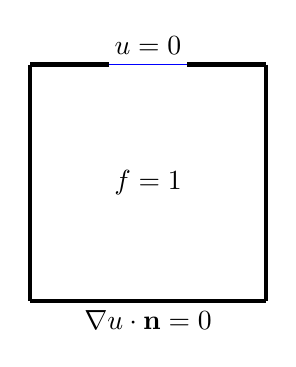
\begin{tikzpicture}
        \draw [ultra thick] (0,0) -- (0,3);
        \draw [ultra thick] (0,0) -- (3,0);
        \draw [ultra thick] (3,3) -- (2,3);
        \draw [blue] (2,3) -- (1,3);
        \draw [ultra thick] (1,3) -- (0,3);
        \draw [ultra thick] (3,3) -- (3,0);

        \node at (1.5, 3) [anchor = south] {$u = 0$};
        \node at (1.5, 1.5) {$f = 1$};
        \node at (1.5, 0) [anchor = north] {$\nabla u \cdot \mathbf{n} = 0$};
    \end{tikzpicture}
\end{figure}
Briefly on the physicality of the solution, first, note that the problem can be interpreted as the construction
of a heat sink within $\Omega$ for which we specify heating loads and where the heat is to dissipate out to, in
this case the load being uniform and constant over $\Omega$ (ie, the heating that the heat sink is subjected to
is uniform throughout the domain) with the heat being able to dissipate out one end.

We see, generally, the sort of surface area maximization that intuition would serve with the tree-like branching,
just as we observe the presence of triangles in solutions to the \texttt{top88.jl} structural compliance problems.


\subsubsection{Unit Square with Two Sinks}

Here, we allow for heat to escape also through a second port; due to the homogeneous boundary conditions, we end up with
an identical problem excepting the boundary condition specification (ie, there are still no boundary terms). This amounts
to a minor change in the boundary element labeling in the implementation (ie, that the lower third must now also be
identified with the same attribute as the top third).

\begin{figure}[H]
    \centering
    \caption[b]{$\Omega$ with two sinks.}
    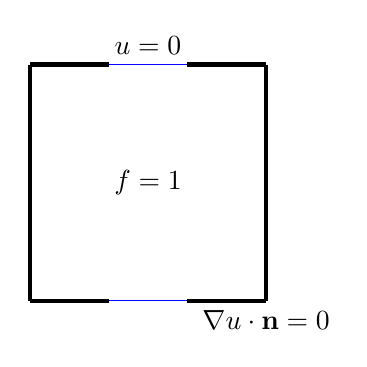
\begin{tikzpicture}
        \draw [ultra thick] (0,0) -- (0,3);

        \draw [ultra thick] (0,0) -- (1,0);
        \draw [blue] (1,0) -- (2,0);
        \draw [ultra thick] (2,0) -- (3,0);

        \draw [ultra thick] (3,3) -- (2,3);
        \draw [blue] (2,3) -- (1,3);
        \draw [ultra thick] (1,3) -- (0,3);

        \draw [ultra thick] (3,3) -- (3,0);

        \node at (1.5, 3) [anchor = south] {$u = 0$};
        \node at (1.5, 1.5) {$f = 1$};
        \node at (3, 0) [anchor = north] {$\nabla u \cdot \mathbf{n} = 0$};
    \end{tikzpicture}
\end{figure}


\vfill\pagebreak

\begin{figure}[H]
    \centering
    \caption{Unit Square with Single Sink: Filtered Distribution}
    \begin{subfigure}{.4\textwidth}
        \includegraphics[width=\textwidth]{imgs/UnitSquare_1/first.png}
        \caption{$t = 1$}
    \end{subfigure}
    \begin{subfigure}{.4\textwidth}
        \includegraphics[width=\textwidth]{imgs/UnitSquare_1/second.png}
        \caption{$t = 6$}
    \end{subfigure}
    \begin{subfigure}{.4\textwidth}
        \includegraphics[width=\textwidth]{imgs/UnitSquare_1/third.png}
        \caption{$t = 13$}
    \end{subfigure}
    \begin{subfigure}{.4\textwidth}
        \includegraphics[width=\textwidth]{imgs/UnitSquare_1/fourth.png}
        \caption{$t = 20$}
    \end{subfigure}
    \begin{subfigure}{.4\textwidth}
        \includegraphics[width=\textwidth]{imgs/UnitSquare_1/fifth.png}
        \caption{$t = 27$}
    \end{subfigure}
    \begin{subfigure}{.4\textwidth}
        \includegraphics[width=\textwidth]{imgs/UnitSquare_1/sixth.png}
        \caption{$t = 35$}
    \end{subfigure}
    \begin{subfigure}{.4\textwidth}
        \includegraphics[width=\textwidth]{imgs/UnitSquare_1/seventh.png}
        \caption{$t = 51$}
    \end{subfigure}
    \begin{subfigure}{.4\textwidth}
        \includegraphics[width=\textwidth]{imgs/UnitSquare_1/eighth.png}
        \caption{$t = 65$}
    \end{subfigure}
\end{figure}

\vfill\pagebreak

\begin{figure}[H]
    \centering
    \caption{Unit Square with Single Sink: State Solution}
    \begin{subfigure}{.4\textwidth}
        \includegraphics[width=\textwidth]{imgs/UnitSquare1_State/first.png}
        \caption{$t = 1$}
    \end{subfigure}
    \begin{subfigure}{.4\textwidth}
        \includegraphics[width=\textwidth]{imgs/UnitSquare1_State/second.png}
        \caption{$t = 6$}
    \end{subfigure}
    \begin{subfigure}{.4\textwidth}
        \includegraphics[width=\textwidth]{imgs/UnitSquare1_State/third.png}
        \caption{$t = 13$}
    \end{subfigure}
    \begin{subfigure}{.4\textwidth}
        \includegraphics[width=\textwidth]{imgs/UnitSquare1_State/fourth.png}
        \caption{$t = 20$}
    \end{subfigure}
    \begin{subfigure}{.4\textwidth}
        \includegraphics[width=\textwidth]{imgs/UnitSquare1_State/fifth.png}
        \caption{$t = 27$}
    \end{subfigure}
    \begin{subfigure}{.4\textwidth}
        \includegraphics[width=\textwidth]{imgs/UnitSquare1_State/sixth.png}
        \caption{$t = 35$}
    \end{subfigure}
    \begin{subfigure}{.4\textwidth}
        \includegraphics[width=\textwidth]{imgs/UnitSquare1_State/seventh.png}
        \caption{$t = 51$}
    \end{subfigure}
    \begin{subfigure}{.4\textwidth}
        \includegraphics[width=\textwidth]{imgs/UnitSquare1_State/eighth.png}
        \caption{$t = 65$}
    \end{subfigure}
\end{figure}

\vfill\pagebreak

\begin{figure}[H]
    \centering
    \caption{Unit Square with Two Sinks: Filtered Distribution}
    \begin{subfigure}{.4\textwidth}
        \includegraphics[width=\textwidth]{imgs/UnitSquare2/first.png}
        \caption{$t = 2$}
    \end{subfigure}
    \begin{subfigure}{.4\textwidth}
        \includegraphics[width=\textwidth]{imgs/UnitSquare2/second.png}
        \caption{$t = 16$}
    \end{subfigure}
    \begin{subfigure}{.4\textwidth}
        \includegraphics[width=\textwidth]{imgs/UnitSquare2/third.png}
        \caption{$t = 32$}
    \end{subfigure}
    \begin{subfigure}{.4\textwidth}
        \includegraphics[width=\textwidth]{imgs/UnitSquare2/fourth.png}
        \caption{$t = 48$}
    \end{subfigure}
    \begin{subfigure}{.4\textwidth}
        \includegraphics[width=\textwidth]{imgs/UnitSquare2/fifth.png}
        \caption{$t = 64$}
    \end{subfigure}
    \begin{subfigure}{.4\textwidth}
        \includegraphics[width=\textwidth]{imgs/UnitSquare2/sixth.png}
        \caption{$t = 80$}
    \end{subfigure}
    \begin{subfigure}{.4\textwidth}
        \includegraphics[width=\textwidth]{imgs/UnitSquare2/seventh.png}
        \caption{$t = 96$}
    \end{subfigure}
    \begin{subfigure}{.4\textwidth}
        \includegraphics[width=\textwidth]{imgs/UnitSquare2/eighth.png}
        \caption{$t = 127$}
    \end{subfigure}
\end{figure}

\vfill\pagebreak

\begin{figure}[H]
    \centering
    \caption{Unit Square with Two Sinks Simulation: State Solution}
    \begin{subfigure}{.4\textwidth}
        \includegraphics[width=\textwidth]{imgs/UnitSquare2_State/first.png}
        \caption{$t = 2$}
    \end{subfigure}
    \begin{subfigure}{.4\textwidth}
        \includegraphics[width=\textwidth]{imgs/UnitSquare2_State/second.png}
        \caption{$t = 16$}
    \end{subfigure}
    \begin{subfigure}{.4\textwidth}
        \includegraphics[width=\textwidth]{imgs/UnitSquare2_State/third.png}
        \caption{$t = 32$}
    \end{subfigure}
    \begin{subfigure}{.4\textwidth}
        \includegraphics[width=\textwidth]{imgs/UnitSquare2_State/fourth.png}
        \caption{$t = 48$}
    \end{subfigure}
    \begin{subfigure}{.4\textwidth}
        \includegraphics[width=\textwidth]{imgs/UnitSquare2_State/fifth.png}
        \caption{$t = 64$}
    \end{subfigure}
    \begin{subfigure}{.4\textwidth}
        \includegraphics[width=\textwidth]{imgs/UnitSquare2_State/sixth.png}
        \caption{$t = 80$}
    \end{subfigure}
    \begin{subfigure}{.4\textwidth}
        \includegraphics[width=\textwidth]{imgs/UnitSquare2_State/seventh.png}
        \caption{$t = 96$}
    \end{subfigure}
    \begin{subfigure}{.4\textwidth}
        \includegraphics[width=\textwidth]{imgs/UnitSquare2_State/eighth.png}
        \caption{$t = 127$}
    \end{subfigure}
\end{figure}

\vfill\pagebreak

\subsubsection{$L$-shaped Domain with a Single Sink}

Here, now over an $L$-shaped domain, we allow for heat to escape part of the left edge. The interior is
also constantly and uniformly heated.

\begin{figure}[H]
    \centering
    \caption[b]{$L$-shaped $\Omega$ with a sink.}
    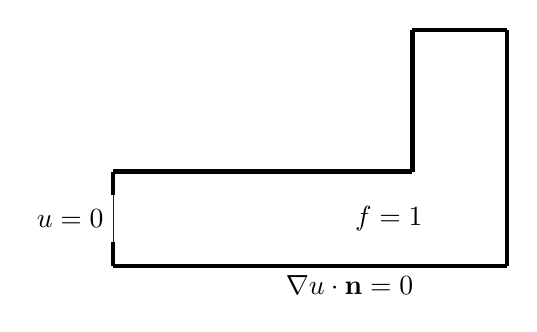
\begin{tikzpicture}
        \draw [ultra thick] (0,0) -- (5,0);
        \draw [ultra thick] (5,0) -- (5,3);
        \draw [ultra thick] (5,3) -- (3.8,3);
        \draw [ultra thick] (3.8,3) -- (3.8,1.2);
        \draw [ultra thick] (3.8,1.2) -- (0,1.2);
        
        \draw [ultra thick] (0,1.2) -- (0,0.9);
        \draw [blue] (0,0.9) -- (0,0.3);
        \draw [ultra thick] (0,0.3) -- (0,0);

        \node at (0, 0.6) [anchor = east] {$u = 0$};
        \node at (3.5, 0.6) {$f = 1$};
        \node at (3, 0) [anchor = north] {$\nabla u \cdot \mathbf{n} = 0$};
    \end{tikzpicture}
\end{figure}

See

\subsubsection{$L$-shaped Domain with a Sink and a Source}

We will allow for heat to escape part of the left edge and enter through part of the top edge (marked red). The interior is no
longer constantly heated, with the source providing the heating instead. The implementation amounts to adding a boundary integrator
for the segment with non-homogeneous boundary conditions.

\begin{figure}[H]
    \centering
    \caption[b]{$L$-shaped $\Omega$ with a sink and a source.}
    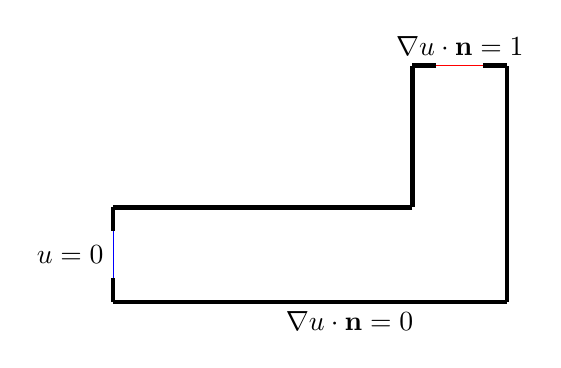
\begin{tikzpicture}
        \draw [ultra thick] (0,0) -- (5,0);
        \draw [ultra thick] (5,0) -- (5,3);

        \draw [ultra thick] (5,3) -- (4.7,3);
        \draw [red] (4.7,3) -- (4.1,3);
        \draw [ultra thick] (4.1,3) -- (3.8,3);

        \draw [ultra thick] (3.8,3) -- (3.8,1.2);
        \draw [ultra thick] (3.8,1.2) -- (0,1.2);
        
        \draw [ultra thick] (0,1.2) -- (0,0.9);
        \draw [blue] (0,0.9) -- (0,0.3);
        \draw [ultra thick] (0,0.3) -- (0,0);

        \node at (0, 0.6) [anchor = east] {$u = 0$};
        %\node at (3.5, 0.6) {$f = 1$};
        \node at (3, 0) [anchor = north] {$\nabla u \cdot \mathbf{n} = 0$};
        \node at (4.4, 3) [anchor = south] {$\nabla u \cdot \mathbf{n} = 1$};
    \end{tikzpicture}
\end{figure}
\vfill\pagebreak



\vfill\pagebreak





\printbibliography

\appendix
\section{\texttt{toph.jl} Derivation and Details}\label{sec:toph_appendix}
See \autoref{lst:toph} for the implementation; here, we will work through the details to the code. \texttt{toph.jl}
is a direct translation
into Julia of the \texttt{toph} listing from the appendices in \cite{bendsoe_sigmund_topopt}. Due to Julia's
design and syntax, the codes end up being quite similar, though the Julia version may be more
familiar to a generally experienced programmer.

The problem is to minimize the thermal compliance in the unit square as was done in \autoref{sec:thermal_compliance_classic_unit_square}.
We are interested in the distribution of two material phases with isotropic conductivities of $1$ and $0.001$ for material and void, respectively.
%\begin{equation}\label{eq:toph_problem}
    %\begin{aligned}
        %\min_{\mathbf{x}} &\quad c(\mathbf{x}) := U^T K U = \sum E_e(x_e) u_e^T k_0 u_e\\
        %\text{s.t.} &\quad V(x)/ V_0 = \theta,\\
            %&\quad KU = F,\\
            %&\quad 0 \leq \rho \leq 1.
    %\end{aligned}
%\end{equation}




\subsection{Primary Loop}
The main optimization loop is as follows:
\begin{algorithm}
    \caption{\texttt{toph}: Main loop.}\label{alg:toph_main}
    \begin{algorithmic}
    \Require \texttt{nelx} (number of $x$ elements), \texttt{nely}, $\theta$ (volume fraction), $p$ (penalization factor), $r_{\text{min}}$ (filter radius)
    \Ensure $x$ satisfies the optimization problem.

    \State $x \gets \theta \cdot \mathbf{1}$ \Comment{Initial guess is a matrix of $\theta$'s}

    \While{not converged}

        $x_\text{old} \gets x$

        $U \gets$ \texttt{FE}; Displacement vector. \Comment{State solution.}

        $KE \gets$ Element Stiffness Matrix

        $c \gets$ objective function calculation

        $dc \gets$ \texttt{check} \Comment{Sensitivity filter.}

        $x \gets$ \texttt{OC} \Comment{Design update step (by the optimality criteria method).}

    \EndWhile
    \end{algorithmic}
\end{algorithm}

The convergence condition depends on the largest value in the difference $x - x_\text{old}$ or the maximum number of allowed iterations.
Here, the only calculation that requires motivation is that of the objective function (the large \texttt{for} loop).
We have seen that this is $U^T K U = \sum E_e(x_e) u_e^T k_0 u_e$. Due to the symmetry between all the square elements, for solid material,
$k_0$ (the element stiffness matrix) is identical,\footnote{The MATLAB code keeps this as a subroutine that returns a constant value,
but this is inefficient in general for several reasons, especially for a JIT language like Julia.} so we need only construct it once and can maintain it as e.g. a \texttt{const}.
\begin{equation}
    KE = \begin{pmatrix}
        k_{11} & k_{12} & k_{13} & k_{14} \\
        k_{21} & k_{22} & k_{23} & k_{24} \\
        k_{31} & k_{32} & k_{33} & k_{34} \\
        k_{41} & k_{42} & k_{43} & k_{44} \\
    \end{pmatrix} = \begin{pmatrix}
        2/3 & -1/6 & -1/3 & -1/6 \\
        -1/6 & 2/3 & -1/6 & -1/6 \\
        -1/3 & -1/6 & 2/3 & -1/6 \\
        -1/6 & -1/3 & -1/6 & 2/3 \\
    \end{pmatrix}.
\end{equation}
We calculate also the sensitivites $\frac{\partial c}{\partial x_e}$, the formula for which we have essentially seen; in particular,
notice that the derivatives are always negative, meaning that increasing the material reduces the thermal compliance of the structure.
\begin{equation}
    \partial c / \partial x_e = -0.999 \cdot p \cdot x_e^{p-1} u^T k_0 u
\end{equation}
\texttt{Ue} denotes the element displacement; obtaining this is a matter of vertex indexation once we have the global displacement vector
\texttt{U}. The elements are numbered column-wise from left to right. This constructed sensitivity matrix is passed into the sensitivity filter subroutine as well as the relevant parameters and current
material distribution.

\subsection{Finite Element Analysis}

We form the global stiffness matrix \texttt{K} with a loop over all elements. Then, the load is set to all $0.01$, meaning that entire domain is
uniformly heated. Finally, the matrix problem $Ku = f$ is solved and the solution $U$ is returned.

\subsection{OC based optimizer}

Here, we follow the algorithm outlined in the discussion of \texttt{top88}; nothing changes in this case with the physics hot-swap. The primary
loop is the bisectioning algorithm for finding the Lagrange multiplier, and while we wait for the bisectioning algorithm, at each step, we update
the distribution in \texttt{xnew}, which is finally returned upon convergence.

\subsection{Mesh-independency filtering}

This is an implementation of the sensitivity filter, which was skipped for the sake of brevity. The scheme modifies the element sensitivities
of the compliance with\cite{bendsoe_sigmund_topopt}
\begin{equation}
    \hat{\frac{\partial f}{\partial \rho_k}} = \frac{1}{\rho_k \sum \hat{H}_i} \sum \hat{H}_i \rho_i \frac{f}{\rho_i},
\end{equation}
where the weight factor $\hat{H}_i$ is
\begin{equation}
    \hat{H}_i = r_\text{min} - \text{dist}(k,i), \quad \{i \in N | \text{dist}(k,i) \leq r_\text{min}\}, k = 1, \ldots, N,
\end{equation}
where $N$ is the number of elements in the mesh.






\section{Julia Code Listings}\label{sec:Julia_Listings}
The following are Julia versions of \texttt{top88} and \texttt{toph}.

\begin{lstlisting}[language=Julia, title=\texttt{top88.jl}, label={lst:top88}]
module Top88

using LinearAlgebra
using SparseArrays
using Statistics

export top88
export prepare_filter
export OC

"""
    top88(nelx, nely, volfrac, penal, rmin, ft)

A direct, naive Julia port of Andreassen et al. "Efficient topology optimization in MATLAB
using 88 lines of code." By default, this will reproduce the optimized MBB beam from Sigmund
(2001).

# Arguments
- `nelx::S`: Number of elements in the horizontal direction
- `nely::S`: Number of elements in the vertical direction
- `volfrac::T`: Prescribed volume fraction
- `penal::T`: The penalization power
- `rmin::T`: Filter radius divided by the element size
- `ft::Bool`: Choose between sensitivity (if true) or density filter (if false). Defaults
    to sensitivity filter.
- `write::Bool`: If true, will write out iteration number, changes, and density for each
    iteration. Defaults for false.
- `loop_max::Int`: Explicitly set the maximum number of iterations. Defaults to 1000.

# Returns
- `Matrix{T}`: Final material distribution, represented as a matrix
"""
function top88(
    nelx::S=60,
    nely::S=20,
    volfrac::T=0.5,
    penal::T=3.0,
    rmin::T=2.0,
    ft::Bool=true,
    write::Bool=false,
    loop_max::Int=1000
) where {S <: Integer, T <: AbstractFloat}
    # Physical parameters
    E0 = 1; Emin = 1e-9; nu = 0.3;

    # Prepare finite element analysis
    A11 = [12  3 -6 -3;  3 12  3  0; -6  3 12 -3; -3  0 -3 12]
    A12 = [-6 -3  0  3; -3 -6 -3 -6;  0 -3 -6  3;  3 -6  3 -6]
    B11 = [-4  3 -2  9;  3 -4 -9  4; -2 -9 -4 -3;  9  4 -3 -4]
    B12 = [ 2 -3  4 -9; -3  2  9 -2;  4  9  2  3; -9 -2  3  2]
    KE = 1/(1-nu^2)/24*([A11 A12;A12' A11]+nu*[B11 B12;B12' B11])

    nodenrs = reshape(1:(1+nelx)*(1+nely),1+nely,1+nelx)
    edofVec = reshape(2*nodenrs[1:end-1,1:end-1].+1, nelx*nely, 1)
    edofMat = zeros(Int64, nelx*nely, 8)

    offsets = [0 1 2*nely.+[2 3 0 1] -2 -1]
    for i = 1:8
        for j = 1:nelx*nely
            edofMat[j,i]= edofVec[j] + offsets[i]
        end
    end

    iK = reshape(kron(edofMat,ones(8,1))', 64*nelx*nely,1)
    jK = reshape(kron(edofMat,ones(1,8))', 64*nelx*nely,1)
    
    # Loads and supports
    F = spzeros(2*(nely+1)*(nelx+1))
    F[2,1] = -1
    U = spzeros(2*(nely+1)*(nelx+1))

    fixeddofs = union(1:2:2*(nely+1), [2*(nelx+1)*(nely+1)])
    alldofs = 1:2*(nely+1)*(nelx+1)
    freedofs = setdiff(alldofs, fixeddofs)

    # Prepare the filter
    H, Hs = prepare_filter(nelx, nely, rmin)
    
    # Initialize iteration
    x = volfrac*ones(nely,nelx)
    xPhys = x
    loop = 0
    change = 1
    cValues = []

    # Start iteration
    while change > 0.01
        loop += 1
        # FE-Analysis
        sK = [j*((i+Emin)^penal) for i in ((E0-Emin)*xPhys[:]') for j in KE[:]]
        K = sparse(iK[:], jK[:], sK)
        K = (K+K')/2

        KK = cholesky(K[freedofs,freedofs])
        U[freedofs] = KK \ F[freedofs]
        
        # OLD: edM = [convert(Int64,i) for i in edofMat]
        mat = (U[edofMat]*KE).*U[edofMat]

        # Objective function and sensitivity analysis
        ce = reshape([sum(mat[i,:]) for i = 1:(size(mat)[1])],nely,nelx)
        c = sum(sum((Emin*ones(size(xPhys)).+(xPhys.^penal)*(E0-Emin)).*ce))
        push!(cValues,c)
        dc = -penal*(E0-Emin)*xPhys.^(penal-1).*ce
        dv = ones(nely,nelx)
        
        # Filtering/ modification of sensitivities
        if ft
            dc[:] = H*(x[:].*dc[:])./Hs./max(1e-3,maximum(x[:]))
        else
            dc[:] = H*(dc[:]./Hs)
            dv[:] = H*(dv[:]./Hs)
        end

        # Optimality criteria update of design variables and physical densities
        xnew = OC(nelx, nely, x, volfrac, dc, dv, xPhys, ft)

        change = maximum(abs.(x-xnew))
        x = xnew

        write && println("Loop = ", loop, ", Change = ", change ,", c = ", c, ", structural density = ", mean(x))
        loop >= loop_max && break       
    end

    return x
end


"""
Prepare sensitivity/ density filter
"""
function prepare_filter(nelx::S, nely::S, rmin::T) where {S <: Integer, T <: AbstractFloat}
    iH = ones(nelx*nely*(2*(convert(Int64,ceil(rmin)-1))+1)^2)
    jH = ones(size(iH))
    sH = zeros(size(iH))
    k = 0
    for i1 = 1:nelx
        for j1 = 1:nely
            e1 = (i1-1)*nely+j1
            for i2 = max(i1-(ceil(rmin)-1),1):min(i1+(ceil(rmin)-1),nelx)
                for j2 = max(j1-(ceil(rmin)-1),1):min(j1+(ceil(rmin)-1),nely)
                    e2 = (i2-1)*nely+j2
                    k += 1
                    iH[k] = e1
                    jH[k] = e2
                    sH[k] = max(0,rmin-sqrt((i1-i2)^2+(j1-j2)^2))
                end
            end
        end
    end
    H = sparse(iH,jH,sH)
    Hs = [sum(H[i,:]) for i = 1:(size(H)[1])]

    return H, Hs
end

"""
Optimality criteria update
"""
function OC(
    nelx::S,
    nely,
    x,
    volfrac,
    dc::Matrix{T},
    dv,
    xPhys::Matrix{T},
    ft::Bool
) where {S <: Integer, T <: AbstractFloat}
    l1 = 0; l2 = 1e9; move = 0.2
    xnew = zeros(nely, nelx)

    while (l2-l1)/(l1+l2) > 1e-3
        lmid = 0.5*(l2+l1)
        RacBe = sqrt.(-dc./dv/lmid)
        XB = x.*RacBe

        for i = 1:nelx
            for j = 1:nely
                xji = x[j,i]
                xnew[j,i]= max(0.000,max(xji-move,min(1,min(xji+move,XB[j,i]))))
            end
        end  

        if ft
            xPhys = xnew
        else
            xPhys[:] = (H*xnew[:])./Hs
        end

        if sum(xPhys[:]) > volfrac*nelx*nely
            l1 = lmid
        else 
            l2 = lmid 
        end
    end

    return xnew
end

end 
\end{lstlisting}

\begin{lstlisting}[language=Julia, title=\texttt{toph.jl}, label={lst:toph}]
module TopH

using LinearAlgebra
using SparseArrays
using Statistics

export toph
export OC
export check
export FE

"""
    toph(nelx, nely, volfrac, penal, rmin, write, loop_max)

A direct, naive Julia port of the `toph` code listing from "Topology Optimization"
by Martin Bendsoe and Ole Sigmund.

# Arguments
- `nelx::S`: Number of elements in the horizontal direction
- `nely::S`: Number of elements in the vertical direction
- `volfrac::T`: Prescribed volume fraction
- `penal::T`: The penalization power
- `rmin::T`: Filter radius divided by the element size
- `write::Bool`: If true, will write out iteration number, changes, and density
    for each iteration. Defaults to false.
- `loop_max::Int`: Explicitly set the maximum number of iterations. Defaults to 1000.

# Returns
- `Matrix{T}`: Final material distribution, represented as a matrix.
"""
function toph(
    nelx::S,
    nely::S,
    volfrac::T,
    penal::T,
    rmin::T,
    write::Bool=false, 
    loop_max::Int=100
) where {S <: Integer, T <: AbstractFloat}
    # Initialization
    x = volfrac * ones(nely,nelx)
    loop = 0
    change = 1.
    dc = zeros(nely,nelx)

    # Start iteration
    while change > 0.01
        loop += 1
        xold = x
        c = 0.

        # FE Analysis
        U = FE(nelx,nely,x,penal)

        KE = [ 2/3 -1/6 -1/3 -1/6
                -1/6  2/3 -1/6 -1/3
                -1/3 -1/6  2/3 -1/6
                -1/6 -1/3 -1/6  2/3 ]

        # Objective function/ sensitivity analysis
        for ely = 1:nely
            for elx = 1:nelx
                n1 = (nely+1)*(elx-1)+ely
                n2 = (nely+1)* elx   +ely
                Ue = U[[n1; n2; n2+1; n1+1]]

                c += (0.001+0.999*x[ely,elx]^penal)*Ue'*KE*Ue
                dc[ely,elx] = -0.999*penal*(x[ely,elx])^(penal-1)*Ue'*KE*Ue
            end
        end

        # Sensitivity filtering 
        dc = check(nelx,nely,rmin,x,dc)
        # Design update by optimality criteria method
        x  = OC(nelx,nely,x,volfrac,dc)

        # Print out results if desired
        if write
            change = maximum(abs.(x-xold))
            println("Change = ", change, " c = ", c)
        end

        loop >= loop_max && break
    end

    return x
end

"""
    OC(nelx, nely, x, volfrac, dc)

Optimality criteria update

# Arguments
- `nelx::S`: Number of elements in the horizontal direction
- `nely::S`: Number of elements in the vertical direction
- `x::Matrix{T}`: Current material distribution
- `volfrac::T`: Prescribed volume fraction
- `dc::Matrix{T}`: Sensitivity filter

# Returns
- `Matrix{T}`: Updated material distribution

"""
function OC(
    nelx::S,
    nely::S,
    x::Matrix{T},
    volfrac::T,
    dc::Matrix{T}
) where {S <: Integer, T <: AbstractFloat}
    l1 = 0; l2 = 100000; move = 0.2
    xnew = zeros(nely,nelx)

    while (l2-l1) > 1e-4
        lmid = 0.5*(l2+l1)
        RacBe = sqrt.(-dc/lmid)
        XB = x .* RacBe

        for i = 1:nelx
            for j = 1:nely
                xji = x[j,i]
                xnew[j,i]= max(0.001,max(xji-move,min(1,min(xji+move,XB[j,i]))))
            end
        end

        if (sum(sum(xnew)) - volfrac*nelx*nely) > 0
            l1 = lmid
        else
            l2 = lmid
        end
    end

    return xnew
end

"""
    check(nelx, nely, rmin, x, dc)

Mesh independency filter

# Arguments
- `nelx::S`: Number of elements in the horizontal direction
- `nely::S`: Number of elements in the vertical direction
- `rmin::T`: Sensitivity filter radius divided by element size
- `x::Matrix{T}`: Current material distribution
- `dc::Matrix{T}`: Compliance derivatives

# Returns
- `Matrix{T}`: Updated dc
"""
function check(nelx::S,
    nely::S,
    rmin::T,
    x::Matrix{T},
    dc::Matrix{T}
) where {S <: Integer, T <: AbstractFloat}
    dcn=zeros(nely,nelx)

    for i = 1:nelx
        for j = 1:nely
        sum=0.0

        for k = max(i-floor(rmin),1):min(i+floor(rmin),nelx)
            for l = max(j-floor(rmin),1):min(j+floor(rmin),nely)
            l = Int64(l); k = Int64(k)
            fac = rmin-sqrt((i-k)^2+(j-l)^2)
            sum = sum+max(0,fac)
            dcn[j,i] += max(0,fac)*x[l,k]*dc[l,k]
            end
        end

        dcn[j,i] = dcn[j,i]/(x[j,i]*sum)
        end
    end

    return dcn
end

"""
    FE(nelx, nely, x, penal)

Finite element implementation

# Arguments
- `nelx::S`: Number of elements in the horizontal direction
- `nely::S`: Number of elements in the vertical direction
- `x::Matrix{T}`: Current material distribution
- `penal::T`: The penalization power

# Returns
- `Matrix{T}`: Differential equation solution U
"""
function FE(
    nelx::S,
    nely::S,
    x::Matrix{T},
    penal::T
) where {S <: Integer, T <: AbstractFloat}
    KE = [ 2/3 -1/6 -1/3 -1/6
            -1/6  2/3 -1/6 -1/3
            -1/3 -1/6  2/3 -1/6
            -1/6 -1/3 -1/6  2/3 ]

    K = spzeros((nelx+1)*(nely+1), (nelx+1)*(nely+1))
    U = zeros((nely+1)*(nelx+1))
    F = zeros((nely+1)*(nelx+1))
    for elx = 1:nelx
        for ely = 1:nely 
            n1 = (nely+1)*(elx-1)+ely
            n2 = (nely+1)* elx   +ely
            edof = [n1; n2; n2+1; n1+1]
            K[edof,edof] += (0.001+0.999*x[ely,elx]^penal)*KE
        end
    end

    F .= 0.01
    fixeddofs = Int64(nely/2+1-(nely/20)):Int64(nely/2+1+(nely/20))
    alldofs = 1:(nely+1)*(nelx+1)
    freedofs = setdiff(alldofs,fixeddofs)

    U[freedofs] = K[freedofs, freedofs] \ F[freedofs]
    U[fixeddofs] .= 0
    
    return U
end
    
end
\end{lstlisting}



\end{document}